The tests were conducted using 4 nodes connected to a gateway. The nodes were placed one on each shelf of the experimental rig in order to see how the height of the shelf affects movement, 
similar to a tall building. The nodes were securely mounted and calibrated until they were stable enough to not be affected by small vibrations which could corrupt the actual data. 
This would also apply to a real world scenario, where the nodes would need a sturdy mounting place to properly sense relevant vibrations in the structure of the building.

We have conducted 3 test runs by setting the supply voltage for the shake table's motors at different values. The shake table was powered on for 3 seconds during each test run.
\begin{itemize}

\item Test run I at 2V ~\ref{fig:2v}. This test will demonstrate that even when the table is barely vibrating, emulating a small earthquake, the nodes are capable of detecting it.
\item Test run II at 4v ~\ref{fig:4v}. This test simulates a stronger earthquake, which is easier to detect.
\item Test run III at 7v ~\ref{fig:7v}. This test generates powerful vibrations which allow us see if the limit of +/-2G set on the nodes can be reached.
\end{itemize}

\begin{figure}[ht] \centering
  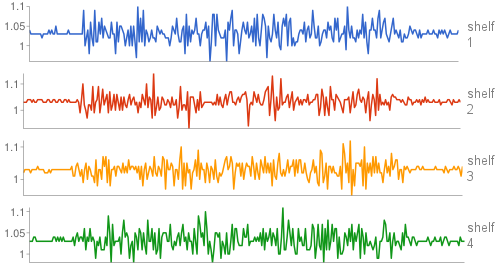
\includegraphics[width=0.5\textwidth]{img/2v.png}
  \caption{Results for the shake table at 2V}
  \label{fig:2v}
\end{figure}

\begin{figure}[ht] \centering
  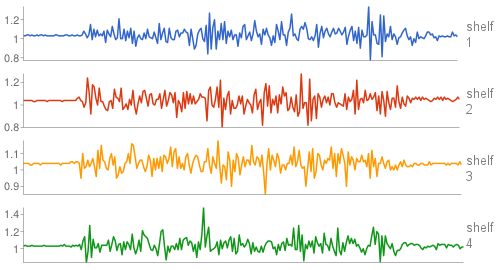
\includegraphics[width=0.5\textwidth]{img/4v.png}
  \caption{Results for the shake table at 4V}
  \label{fig:4v}
\end{figure}

\begin{figure}[ht] \centering
  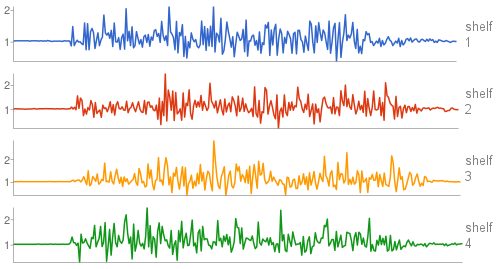
\includegraphics[width=0.5\textwidth]{img/7v.png}
  \caption{Results for the shake table at 7V}
  \label{fig:7v}
\end{figure}

As it can be seen in figure~\ref{fig:2v}, figure~\ref{fig:4v} and figure~\ref{fig:7v}, the value range when the table is still is around 1G with a diference of 0.04G. Any value that is higer or lower than that and is relatively periodical can be interepreted as an eartquake. 

The results prove that the experimental rig is responding similar to a tall building because the lower positioned nodes gather stronger values than the ones located on higher shelves 
when the table is vibrating. At the end of the simulation, when the table is no longer shaken and it is naturaly vibrating due to previous forces, the higher positioned nodes continue 
to detect vibrations, as it should have happened in the case of a real building.
